%---------------------------------------------------------------
\chapter{Additional constraints and detrending\label{chap:advection}}
%---------------------------------------------------------------

This chapter shows how additional dynamical constraints (advection, diffusion, source, decay) can be added to the cost function that provide the analysed field in \diva. It also describes the \textit{detrending} tool, which allows the extraction of trends from groups.

\minitoc


\section{Adding advection to the cost function}
%---------------------------------

Activating an advection \index{Advection}constraint on the tracers is done by adding a term to the norm of the field $\varphi$ \eqref{divaformula2}, leading to

\begin{equation}
\tilde{J}= J(\varphi) + \frac{\theta}{U^2 L^2} \int_{\tilde{D}}\left[
\vect{u} \cdot \tilde{\nabla} \varphi
- \frac{\mathcal{A}}{L} \, \tilde{\nabla}\! \cdot\! \tilde{\nabla}\varphi
\right]^2 \ddiff \tilde{D}
\end{equation}

where $U$ and $L$ are characteristic velocity and length scales, respectively. We recognize a dimensionless version of stationnary advection-diffusion equation

\begin{equation}
\vect{u} \cdot {\nabla} \varphi
~=~ \mathcal{A}  \, {\nabla}\! \cdot\! {\nabla}\varphi 
\end{equation}

The parameter $\theta$ allows one to adapt the weight of the additional second term, in which we recognize a stationary advection-diffusion equation. The physical meaning of the term $\vect{u} \cdot \tilde{\nabla} \varphi$ is simple: when the velocity is nearly parallel to the gradient, the product has a large value and is thus penalized. Then for a strong constraint ($\theta\gg 1$) we enforce the analysis to align with velocity.

In general we can assume $\mathcal{A} \le U L$, in other words, we work at relatively high \textit{Reynolds numbers} \footnote{The Reynolds number measures the ratio of the inertial effects over the viscosity effects}. Otherwise for dominant diffusion, the term just adds another isotropic filtering effect, already included in the regularization term (Eq.~\ref{divaformula2}). Hence the additional term is really interesting only for situations dominated by advection, with $\mathcal{A} \le U L$. In this case, the scaling is such that for $\theta\approx 1$, the advection constraint has a similar importance with respect to the regularization term.

The velocity scale $U$ is calculated from the provided $\vect{u}=(u,v)$ field. 

Note that when using the advection constraint, the correlation length provided by \command{divafit} should be decreased since the advection 
constraint implicitly increases correlation length along currents.

The solution is expanded in terms of so-called connector values (typically values at the nodes of a finite element mesh, and in the present case, also normal derivatives to interfaces) and shape functions over each element (Section~\ref{sec:finiteelements})\index{Finite-elements}. This allows the computation of the solution at any desired location, knowing the connector values.

The connector values themselves are found as the solution of the minimization process:

\begin{equation}
\left( \matr{K}_s + \matr{K}_d \right) \vect{q} = \vect{g}
\end{equation}

The stiffness matrix $\matr{K}=\matr{K}_s + \matr{K}_d$ is composed by the different terms related to the derivatives ($\matr{K}_s$) and a final term related to the location of data:
\begin{equation}
\matr{K}_d ~=~ \sum_{i=1}^{N_d} \mu_i \matr{S}_i \transp{\matr{S}}_i
\end{equation}
where $\matr{S}_i$ is a column vector containing the shape functions associated with a data point $i$. This
vector has zeros everywhere, except for all connectors of the element in which the data point lies.

Similarly, the data value $d_i$ come into the formulation by a projection of the data onto the charge vector of the connectors
\begin{equation}
\vect{g}_i = \mu_i \matr{S}_i d_i
\label{eq:fromdatato}
\end{equation}
and the total charge vector is the sum of the individual ones.

When a constraint is added, in the original version, the stiffness matrix is augmented by components for each element $\Omega$ which are computed
\begin{equation}
\int_\Omega \left( u {\partial s_i \over \partial x}+v {\partial s_i \over \partial y}-\mathcal{A} {\partial^2 s_i \over \partial x^2} -\mathcal{A} {\partial^2 s_i \over \partial y^2}\right) \left( u {\partial s_j \over \partial x}+v {\partial s_j \over \partial y}-\mathcal{A} {\partial^2 s_j \over \partial x^2} -\mathcal{A} {\partial^2 s_j \over \partial y^2}\right)\ddiff \Omega
\end{equation}

where $s_i$ are the shape functions of the element



\subsection{Advection alone}
%------------------------------

Figure~\ref{fig:solidrot} shows an example of a single data point in\, $(0.7,60)$ with unit value in a solid 
rotation (centred in $(0,60)$). In the absence of diffusion, up and downwind are identical (covariance 
counts).

\begin{figure}[H]
\parbox{.6\textwidth}{
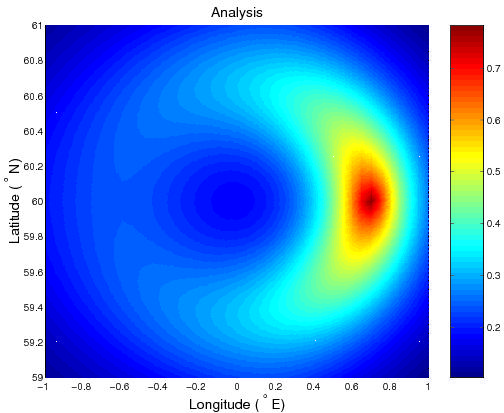
\includegraphics[width=.55\textwidth]{solidrot}
}\parbox{.4\textwidth}{
\caption{Single data point with unit value in a solid 
rotation.\label{fig:solidrot}}
}
\end{figure}


Without advection (Fig.~\ref{fig:norot}), the across velocity scale remains and isotropy is 
recovered (except for boundary effect on the right side).

\begin{figure}[H]
\parbox{.6\textwidth}{
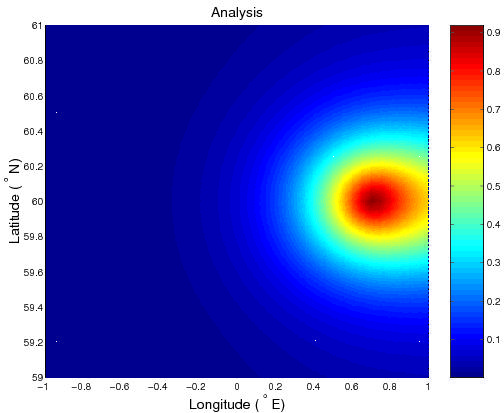
\includegraphics[width=.55\textwidth]{norot}
}\parbox{.4\textwidth}{
\caption{Same as Fig. \ref{fig:solidrot}, but without advection. \label{fig:norot}}
}
\end{figure}



To decrease the across frontal scale, we must decrease $L$ but add advection 
to keep along-current scale larger (Fig. \ref{fig:solidrotsmall}).

\begin{figure}[H]
\parbox{.6\textwidth}{
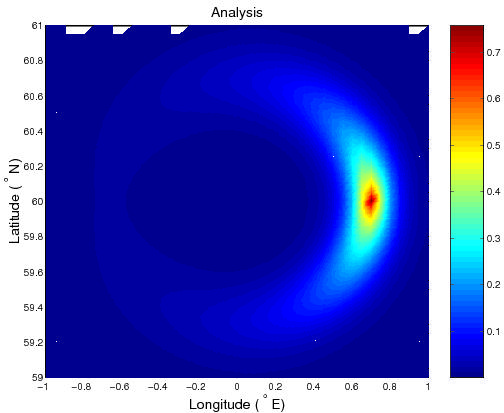
\includegraphics[width=.55\textwidth]{solidrotsmall}
}\parbox{.4\textwidth}{
\caption{Same as Fig. \ref{fig:solidrot}, but with smaller length scale. \label{fig:solidrotsmall}}
}
\end{figure}


Adding advection without decreasing $L$ increases correlation length 
along front and keeps across front correlation length.

%--------------------------------------
\subsection{Advection and diffusion}
%--------------------------------------

Adding diffusion \index{Diffusion} makes possible the distinction between up and downwind 
direction (Fig.~\ref{fig:solidrotp}): in this case, higher values are found upwind of the data 
location: this is natural, because the data is observed and \diva tries to 
infer the field that explains the sample. This requests higher values 
upwind (because downwind values decrease).

Because of the square in the formulation, to change the flow direction 
you can simply change the sign of the diffusion coefficient or change 
the sign of the velocity components (Fig.~\ref{fig:solidrotm}).

\begin{figure}[htpb]
\parbox{.6\textwidth}{
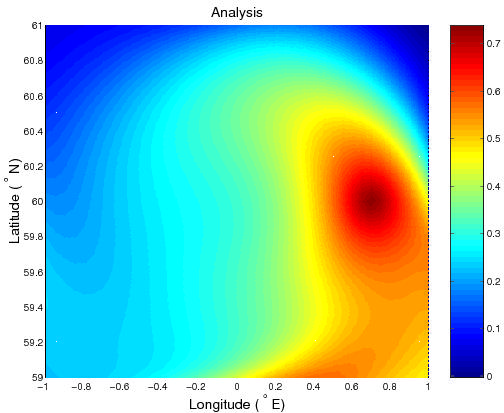
\includegraphics[width=.55\textwidth]{solidrotp}
}\parbox{.4\textwidth}{
\caption{Single data point with anti-clockwise rotation and with diffusion. \label{fig:solidrotp}}
}
\end{figure}

\begin{figure}[htpb]
\centering
\parbox{.6\textwidth}{
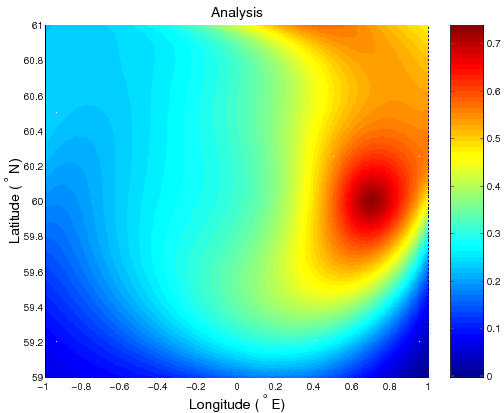
\includegraphics[width=.55\textwidth]{solidrotm}
}\parbox{.4\textwidth}{
\caption{Single data point with clockwise rotation and with diffusion. \label{fig:solidrotm}}
}
\end{figure}


%--------------------------
\subsection{Generalization}
%--------------------------

Zero diffusion simply leads to correlations that are increased in the 
direction of the vector $\vect{u}$ (or decreased in the perpendicular 
direction if the global $L$ is increased simultaneously). 

The vector $\vect{u}$ does not need to be a velocity in this case, but can be any 
vector indicating the direction in which correlation is to be increased.
Hence it could be for example, topography gradients rotated by $90$ degrees 
or density gradients rotated by 90 degrees if we respectively assume across depth-contour movements are more 
difficult (and hence data correlation decreased) or across frontal movements more difficult (and hence correlation length 
across fronts decreased). This idea is implemented in \command{divaUVtopo} which generates a "velocity" field along isobath.

The advection constraint therefore allows any known anisotropy in the correlations to be included into the analysis. We notice that the vector field does not need to be divergence free.

% \subsection{Error field}

% provided by diva, but interpretation different as the normal case
% need to add more details on this

%--------------------------------------
\section{Adding linear sink(s) and local source(s)}
%--------------------------------------
\index{Sinks and sources}
With the more complete equation

\begin{equation}
\vect{u} \cdot {\nabla} \varphi
~=~ \sum_j \mathcal{Q}_j\delta( \vect{\tilde{r}}-\vect{\tilde{r}}_j ) ~-\gamma \varphi ~+ \mathcal{A}  {\nabla}\! \cdot\! {\nabla}\varphi ,
\end{equation}
we augment the functional as

\begin{equation}
\tilde{J}= \tilde{J}_1(\varphi) + {\theta  } \int_{\tilde{D}}\left[ 
\vect{\tilde{u}} \cdot \tilde{\nabla} \varphi
- {1  \over Re} \, \tilde{\nabla}\! \cdot\! \tilde{\nabla}\varphi
 +  \gamma {L \over U}  \varphi   - \sum_j \mathcal{Q}_j {L \over U} \delta( \vect{\tilde{r}}-\vect{\tilde{r}}_j ) \right]^2 \ddiff \tilde{D}.
\end{equation}

%-------------------------
\subsection{Implementation}
%-------------------------


$\matr{K}_s$ is easily modified by adding the decay term during the calculation of the constraint:
\begin{eqnarray}
\int_\Omega \left( u {\partial s_i \over \partial x}+v {\partial s_i \over \partial y}-\mathcal{A} {\partial^2 s_i \over \partial x^2} -\mathcal{A} {\partial^2 s_i \over \partial y^2}+ \gamma s_i \right) \quad \quad \quad \notag \\
\quad \quad \quad \left( u {\partial s_j \over \partial x}+v {\partial s_j \over \partial y}-\mathcal{A} {\partial^2 s_j \over \partial x^2} -\mathcal{A} {\partial^2 s_j \over \partial y^2}
+\gamma s_j
\right)\ddiff \Omega. \notag 
\end{eqnarray}

The source is a little bit more complicated :
each source has a contribution to the charge vector $\vect{g}$ of the type

\begin{equation}
2 \int_\Omega \left( u {\partial s_i \over \partial x}+v {\partial s_i \over \partial y}-\mathcal{A} {\partial^2 s_i \over \partial x^2} -\mathcal{A} {\partial^2 s_i \over \partial y^2}+ \gamma s_i \right) {\mathcal{Q} \over \Omega} \ddiff \Omega
\end{equation}
where $\mathcal{Q}$ is taken constant over the sub-element for simplicity (otherwise we need to calculate the derivatives at the source location instead at the gauss integration points where we know them already).


\begin{itemize}
\item
Each source (unit= unit of tracer by unit time), is spread over sub-element in which source is found.
\item
Source file \file{sources.dat} similar to data file. Read in a similar way and sources sorted in a similar way also (which needed some adaptations)
\item Files modified
\file{solver.f constr.f divainc.h datapr.f divacalc}
\item File added: \file{sourcepr.f}
\item \file{constraint.dat} can now contain a third optional parameter which is $\gamma$.
\end{itemize}

Only two possibilities for coordinates and units:
\begin{itemize}
\item user coordinates ({\tt icoordchange=0}): velocity (L/T), decay rate (1/T), diffusion (L$^2$/T) and decay (1/T) and coordinates (L) must have same units. Source has variable unit over time dimension;
\item coordinates are degrees and are transformed to km ({\tt icoordchange=1}): velocity must be in m/s, diffusion in m$^2$/s, decay in 1/s and source in "variable units"/s
\end{itemize}
Other limitations: 
\begin{itemize}
\item
With decay or source activated, {\tt ireg} should be zero (but is not checked).
\item
Poor man error field is really bad for these cases.
\end{itemize}

%------------------------------------------------------------
%Problem of the source term units: $\varphi$ is normally a concentration and hence the variable under investigation  per surface unit (eg. kg per surface unit). Without coordinate change, the source term should then be in kg per time unit.
%
%With the coordinate change from degrees to km internally  and if we want to keep the same "analysed values" we must assume that standard is kg/m$^{}2$. Hence Q/1E6?? I think so...
%
%Test with just source and no data, but sufficient decay and diffusion and large L


% \begin{itemize}
% \item Checks to do (because of changes in data location and data sorting in parallel with source location and source sorting): no sources, source outside of mesh, several sources, more sources than data, data out of mesh etc
% \item check why 1/L$^2$ in parameter of functional ?? Simply because original version is in dimensional form and in this case one has to add $1/L^2$ the dimensionless version
% \end{itemize}

%-------------------
\subsection{Example}
%-------------------

%\begin{figure}
%\includegraphics[width=\textwidth]{%
%./constraint/diva_analysis.ps}
%\caption{Standard analysis with advection constraint\label{fig:constr}}
%\end{figure}
%\begin{figure}
%\includegraphics[width=\textwidth]{%
%./constraint/diva_analysis_decay.ps}
%\caption{Analysis with advection constraint and decay\label{fig:constrdecay}}
%\end{figure}
%\begin{figure}
%\includegraphics[width=\textwidth]{%
%./constraint/diva_analysis_decay_diff.ps}
%\caption{Analysis with advection constraint, decay and diffusion\label{fig:constrdiff}}
%\end{figure}
%\begin{figure}
%\includegraphics[width=\textwidth]{%
%./constraint/diva_analysis_all.ps}
%\caption{Analysis with advection, diffusion, decay and source\label{fig:constrall}}
%\end{figure}


%-------------------------------------------------------
\section{Detrending data by defining groups and classes\label{sec:detrending}}
%-------------------------------------------------------

When analysing climatological data, one is very often faced with data sets that have heterogeneous coverage in time and/or in space. This can lead to misinterpretations of the analysis, if for example there have been much more measurements during a specially warm year than during other years. It is also not uncommon that there are much less cruise data sets in stormy periods than in calm periods. \index{Detrending}

Here we present a method to deal with such problems by defining \textit{classes} and \textit{groups}.

A \textit{group} is simply one way of subdividing the data into different members. For example a group can be based on years and 
the classes are 1995, 1996, 1997 if we are looking at this period. Another group could be based on seasons and classes could be winter, spring, summer and autumn.

\subsection{Theory}
%------------------

In the functional to be minimised by \diva, there is a data-analysis misfit term :
\begin{equation}
\sum_{i=1}^{N_{d}} =  \mu_i \left[ d_i - \varphi(x_i,y_i) \right]^2
\end{equation}
where $\mu_i$ is the data weight on data $d_i$ found in location $x_i,y_i$. The solution of the minimisation is the analysed field $\varphi(x,y)$.


If we define one group, each data point is in one and only one class $C_j$ of this group. Hence
when calculating the misfit in the minimisation part of \diva , we include now an (unknown) trend value for each class ($d_{C_1}, d_{C_2} ...$):

\begin{equation}
\sum_{i\in C_1} \mu_i \left[ d_i -d_{C_1}- \varphi(x_i,y_i) \right]^2 + \sum_{i\in C_2} \mu_i \left[ d_i -d_{C_2}- \varphi(x_i,y_i) \right]^2 + ...
\end{equation}
If we assume we know the function $\varphi(x,y)$, minimisation with respect to each of the unknowns $d_{C_j}$ yields


\begin{equation}
d_{C_1} ~=~{ \sum_{i\in C_1} \mu_i \left[ d_i - \varphi(x_i,y_i) \right] \over \sum_{i\in C_1} \mu_i }
\end{equation}
and similarly for the other classes. Hence we see that the trend for each class is the weighted misfit of the class with respect to the overall analysis.
The problem is of course that $\varphi$ is not known since it is also the result of the minimisation process. However, we can iterate and start with an analysis without detrending. Then, using the field of $\varphi$, we can calculate a first guess of the trends in each group and subtract if from the original data. 
Then a new analysis can be performed, the trends recalculated and so on until convergence.


\subsection{Implementation}

Here we generalize by allowing several groups of classes.

The detrending is done hierarchically:
\begin{enumerate}
\item Trends for the first group are calculated and removed from the data. 
\item The second group is treated and so on.
\item Once the data has been detrended, a new diva analysis is performed. 
\item With the new analysis, the data-analysis misfit (or residual) can be reused to
calculate better estimates of the trends. 
\end{enumerate}
This loop is repeated a predefined number of times. 

%_--------------------------
\subsection{Generalizations}
%---------------------------

We can further add regularization constraints on the calculated trends. For example, if there a few data available for estimating the trend of class $C_j$, we
should be not be too confident on the trend and rather perform a standard analysis (i.e. reducing the value of $d_{C_j}$). We can modify the
cost function associated with data in class $C_j$ as follows

\begin{equation}
\sum_{i\in C_j} \mu_i \left[ d_i -d_{C_j}- \varphi(x_i,y_i) \right]^2 + \alpha_j (d_{C_j})^2
\end{equation}
where the coefficient $\alpha_j$ regularizes the trend amplitude and
\begin{equation}
d_{C_1} ~=~{ \sum_{i\in C_1} \mu_i \left[ d_i - \varphi(x_i,y_i) \right] \over \sum_{i\in C_1} \mu_i + \alpha_i}
\end{equation}
If $N_j$ is the number of points with non-zero weights, we can define
\begin{equation}
\bar{\mu}_j = {1 \over N_j} \sum_{i\in C_j} \mu_i
\end{equation}
and a proposed scaling for regularization constants is
\begin{equation}
\alpha_j = \bar{\mu}_j \sqrt{N_j}.
\end{equation}
This has been implemented.



If the detrending is included in a 3-D loop, with the same groups and classes defined in each layer, we can further request that the values of the trends in a given layer are not too far from those in the surrounding layers and modify the norm as

\begin{equation}
\sum_{i\in C_j} \mu_i \left[ d_i -d_{C_j}- \varphi(x_i,y_i) \right]^2 + \alpha_j (d_{C_j})^2 + \beta^+ (d^+_{C_j}- d_{C_j})^2 + \beta^- (d^-_{C_j}- d_{C_j})^2
\end{equation}
where the coefficient $\beta_j^*$ regularize the trend differences between layers and where $^+$ refers to the value in the layer above and $^-$ to the layer below. Obviously, the solution of this problem will involve tridiagonal solvers. For the lowest and uppermost layer, we can simply assume a zero gradient for the trends.

Similarly, the $ \beta$ can be scaled based on the two layers involved

\begin{equation}
\beta^+_j = { (\bar{\mu}^+_j N_j^+ + \bar{\mu}_j N_j) \over (N_j^++N_j) }
\end{equation}

This regularisation between layers is not yet implemented. Either done at 3-D level or simply allow iterative 3-D filtering as now but with weights $\beta$ as described here !


%---------------
\subsection{Use}
%---------------

Simply provide \file{./input/data.dat} with additional fifth, sixth \ldots columns. If you do not want to use variable data weight, column 4 must contain the value of 1. Column 5, 6, \ldots contain the information in which class the data point falls. Classes must be numbered starting with 1.

\example
\begin{itemize}
\item
Column 5 contains value 1 for a data point of the year 1975, 2 for 1976, 3 for 1977 and so on.
\item
Column 6 contains 1 for a data corresponding to month 01-03, 2 for the month 04-06 and so on.
\item
Column 7 contains 1 for day values, 2 for night values.
\item
Column 8 contains 1 for points that have a density below 1025~kg/m$^3$, 2 for points that have a density above it.
\end{itemize}

Execute \command{divadetrend ngroups [niterations]}. The parameter {\tt ngroups} specifies that the first {\tt ngroups} will be used for the detrending.
(You might create for exemple 5 groups and try with detrending on the first one only using \command{divadetrend 1}). The optional parameter {\tt niterations} tells how many iterations are to be performed for the detrending. Default value is 10 iterations.

\subsubsection{Outputs}
\file{./output/rmsmisfit.dat} contains the evolution during the iterations of the misfit (after detrending). It should decrease if the detrending works well.  \file{trends.all.1.dat} deals with group 1 and contains on column 1 the class number and on columns 2 the final trend value associated with it. Columns 3 and 4 correspond to the next to last iteration and the last columns to the first iteration.

\command{divagnu} produces plots for the trend in each group.


\paragraph{Notes:} 
\begin{itemize}
\item Presently you can define at maximum 5 groups with each group having 50 classes (members). You can increase these limits by editing and compiling \file{src/Fortran/detrend.f}
\item It is assumed that the mesh already exists, otherwise execute \command{divamesh} before.
\end{itemize}

\subsubsection{Additionnal options}

If you provide file \file{detrend.order} in \directory{./input/}, then the columns for detrending will be taken in the order 
specified in the file. 

\example if \file{detrend.order} contains:
\texttt{
8 5 7 6
}\\
and we call \command{divadetrend 3}, columns \texttt{8 5 7} will be used in this order for detrending. If there is no file \file{detrend.order}, then \command{divadetrend 3} will use 5 6 7 in this order.

(file \file{detrend.order} or default order is written in \file{fort.56} in \directory{divawork} during execution)




%-------------------
\subsection{Interna}	% to be moved in Chapter 17-DivaScriptCode.tex
%-------------------

\texttt{detrend.a} creates a new \file{./input/data.dat}.  

\subsubsection{Input}

\file{fort.88} original data file, \file{fort.89} analysis at data points. 
 
\subsubsection{Output}

\texttt{fort.90} modified data file with data detrended by groups and classes. \file{trends.1.dat} trends for classes of group 1. \file{\tt trends.2.dat} trends for classes of group 2 etc.

\subsection{Example}

The example located in \directory{Examples/Trends/} contains data sampled from a spatial pattern (sin-cosine structure) over which was added: 
\begin{itemize}
\item a seasonal cycle, 
\item a daily cycle and 
\item inter-annual variations.
\end{itemize}

Groups are years, month and hours. Matlab file \file{pseudodata.m} can be used to generated such a data file. The comparison between analysed field without and with detrending option is shown in Fig.~\ref{fig:detrend1}: on the left-hand side, the sin-cosine structure is visible, but perturbed by the various cycles superimposed on it. After the detrending, the structure is perfectly recovered.

\begin{figure}[htpb]
\centering
\subfigure[]{
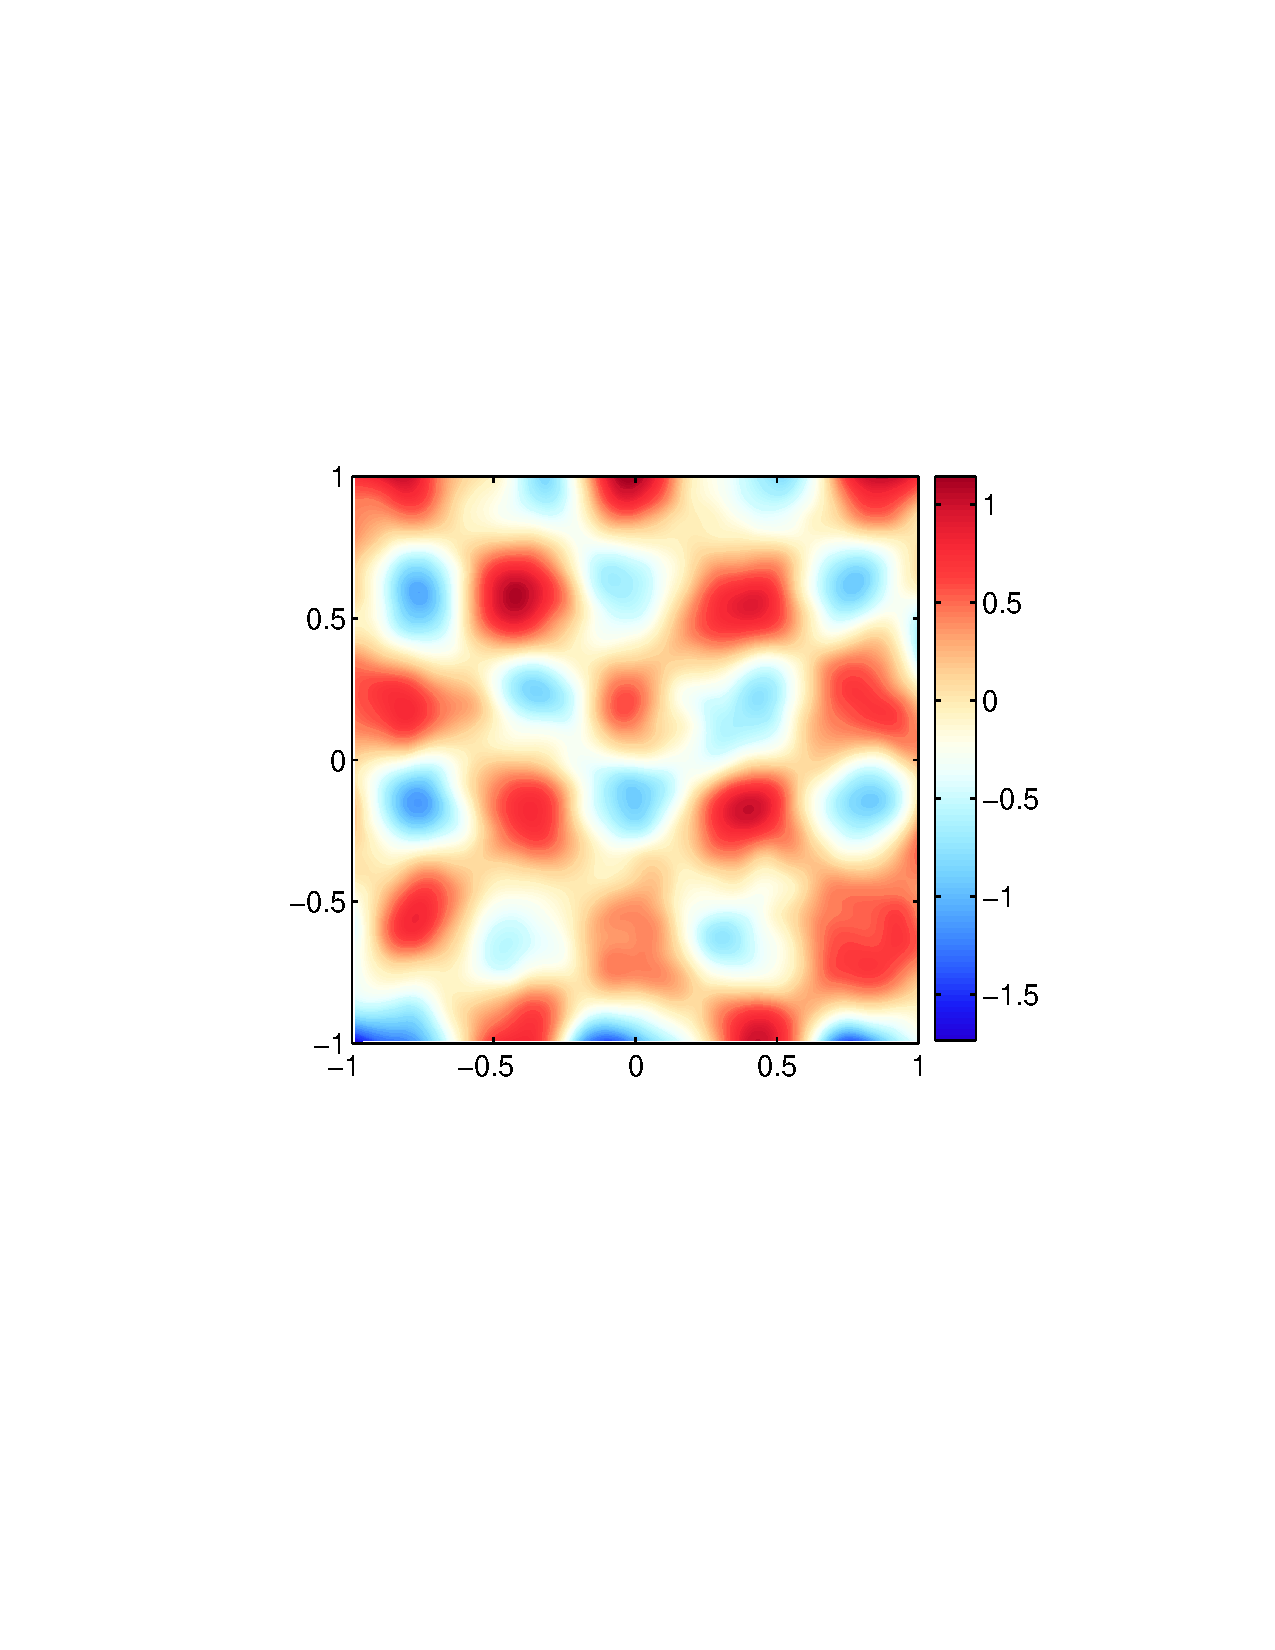
\includegraphics[width=.475\textwidth,bb=136 270 504 575]{analysis_nodetrend}
}\subfigure[]{
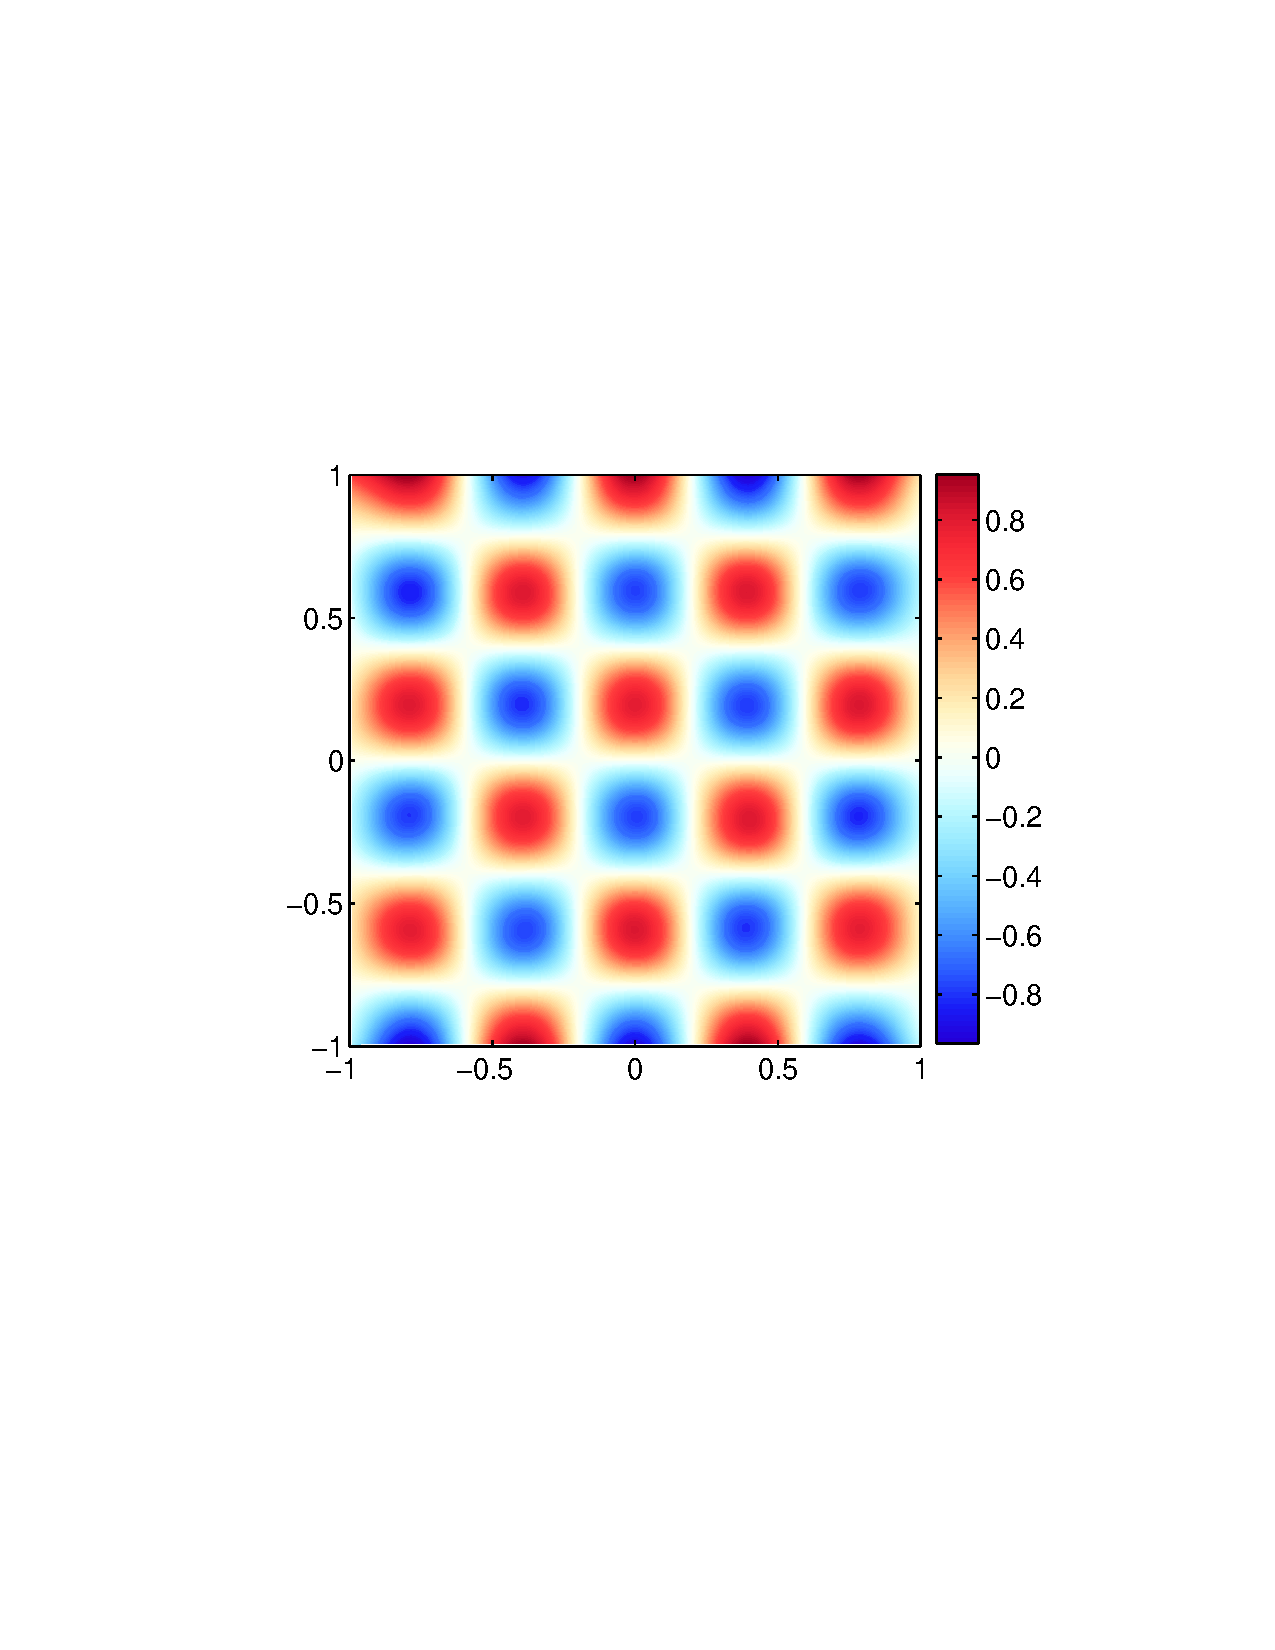
\includegraphics[width=.475\textwidth,bb=136 270 504 575]{analysis_detrend}
}
\caption[Example of a reconstruction without and with detrending.]{Example of a reconstruction without (a) and with detrending (b). Note the difference in the color bars.\label{fig:detrend1}}
\end{figure}

Along with the field without trend, the \command{divadetrend} tool also provides the trend for each group (Fig.~\ref{fig:detrend2}).

\begin{figure}[htpb]
\centering
\subfigure[Inter-annual]{
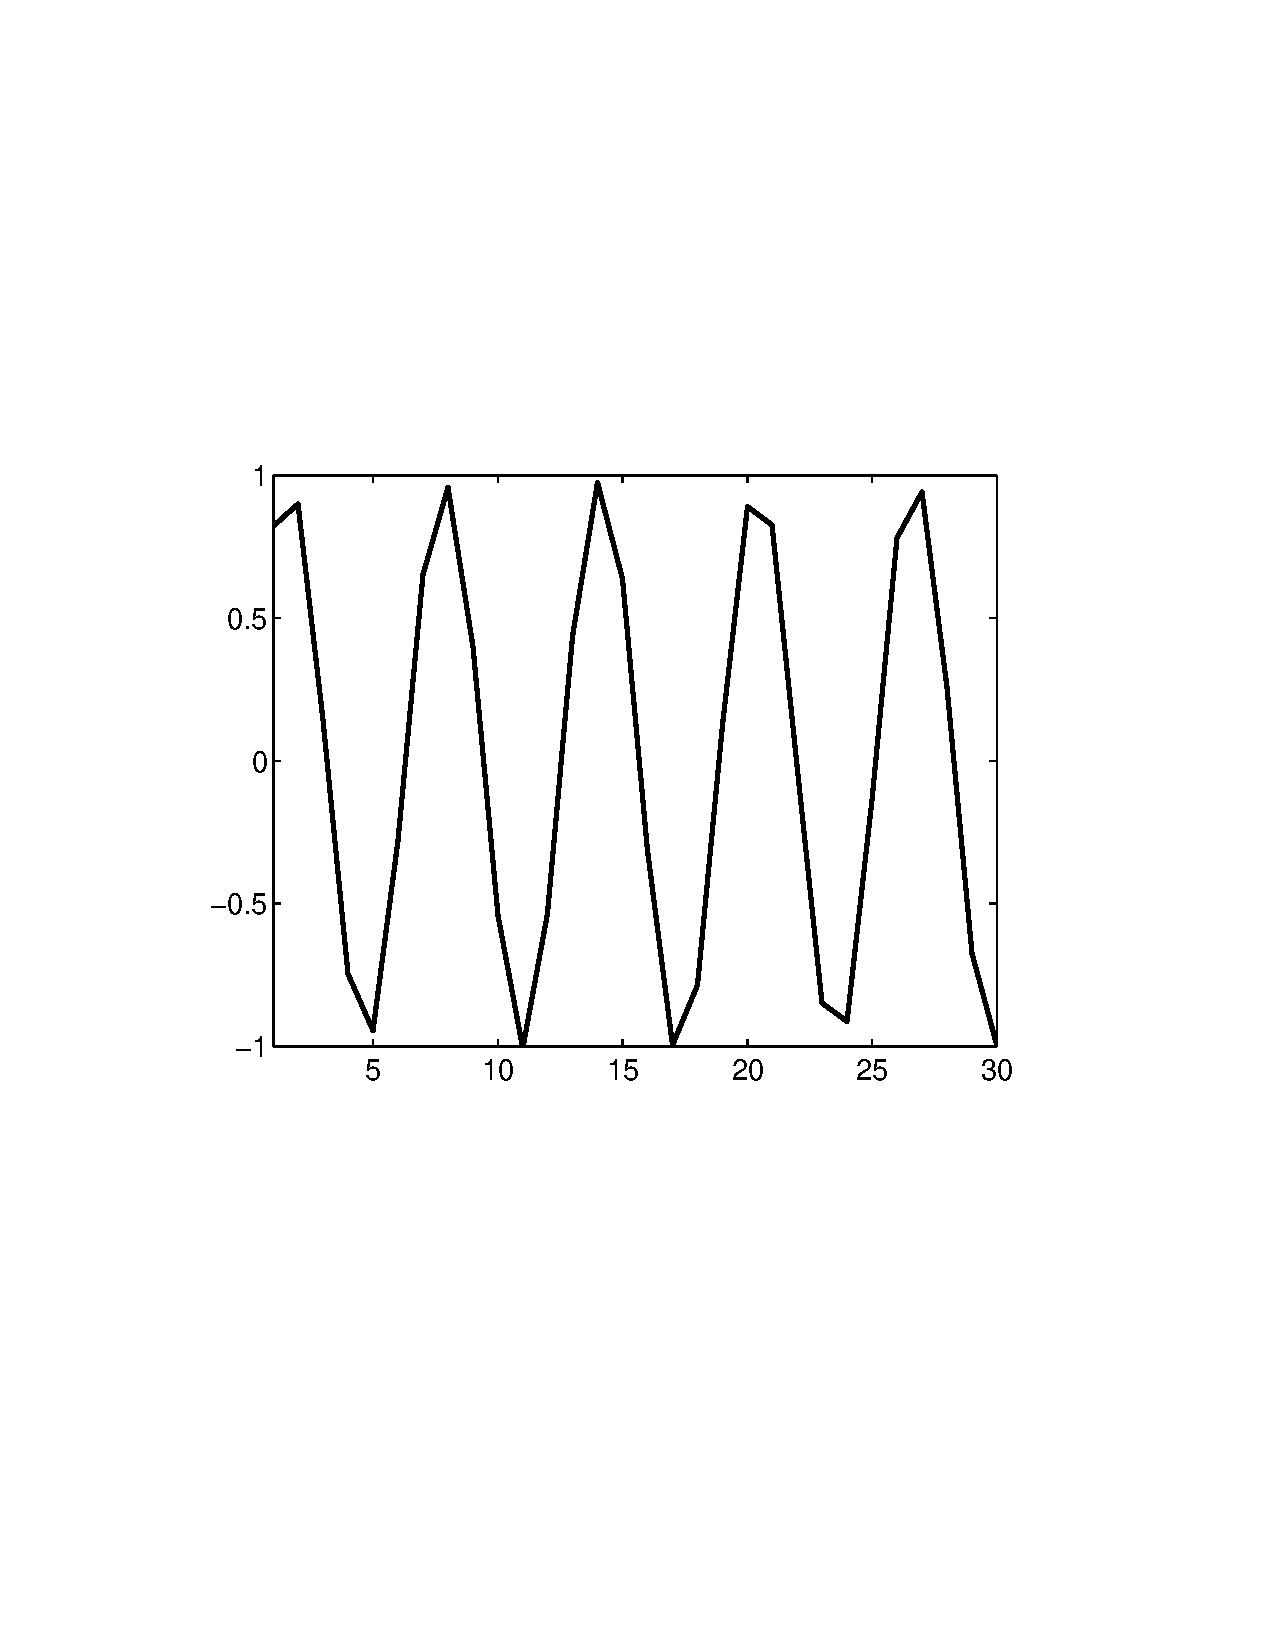
\includegraphics[width=.475\textwidth,bb=100 270 490 575]{example_detrend1}
}\subfigure[Seasonal]{
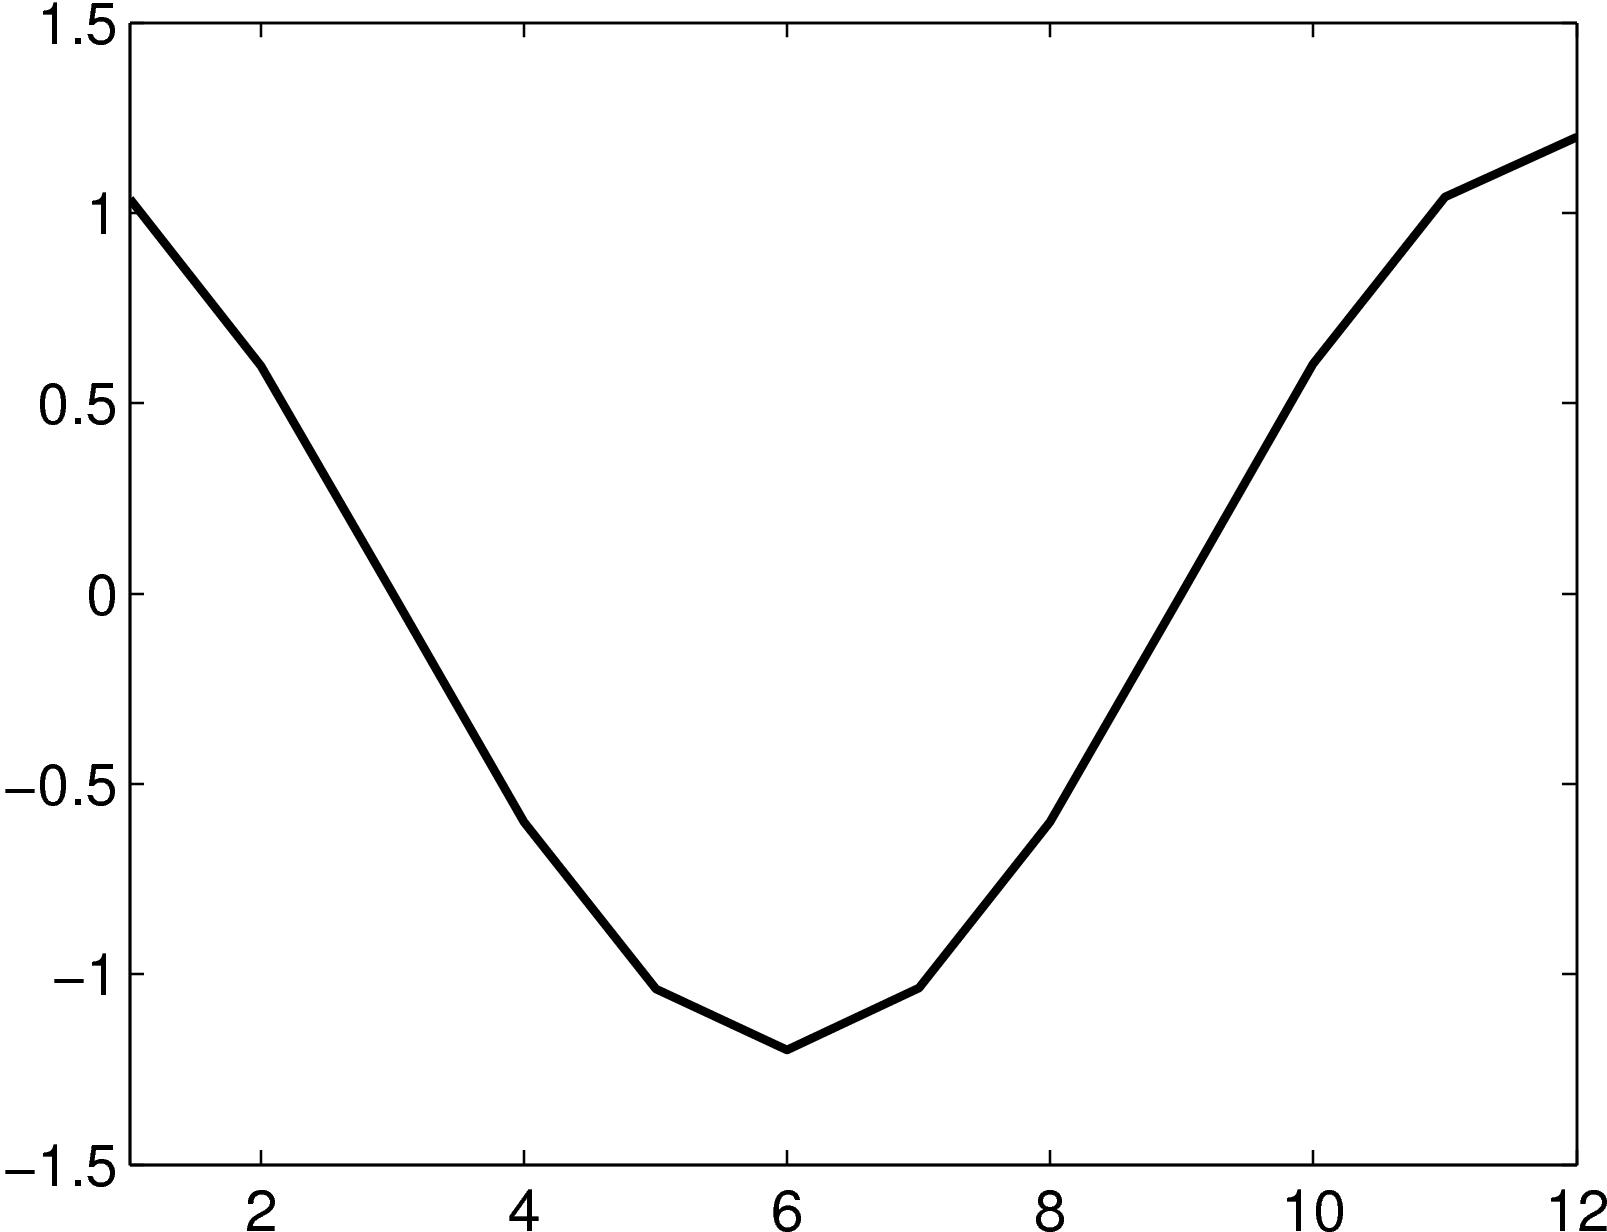
\includegraphics[width=.475\textwidth,bb=100 270 490 575]{example_detrend2}
}
\subfigure[Daily]{
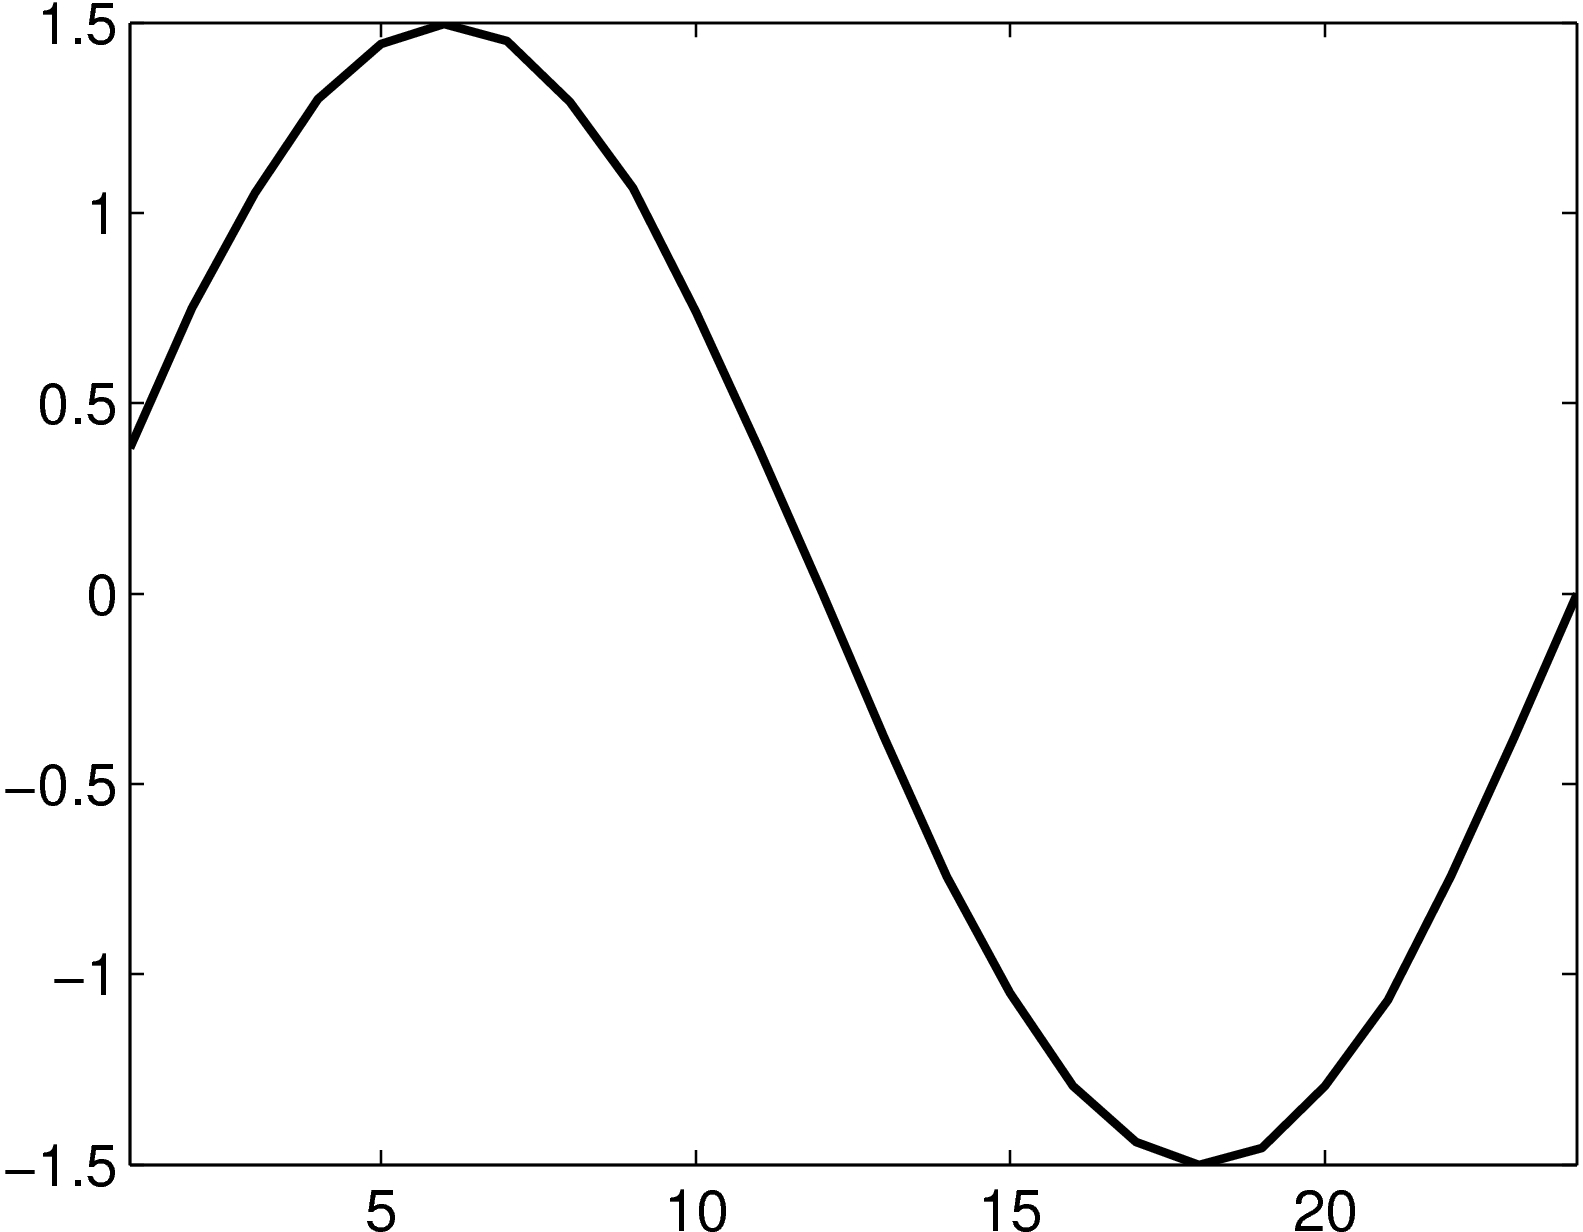
\includegraphics[width=.475\textwidth,bb=100 270 490 575]{example_detrend3}
}
\caption{Trends obtained from the data using the detrending tool.\label{fig:detrend2}}
\end{figure}

% \subsection{Future developments}	%  = things to do!

% Prepare detrending with global south-north gradient (for seasonal cycle). Use variance to diagnose which type of function?
% Include exclusion value to avoid needing eliminating data (simply put weights zero for land points).

% For the 3-D version, pack data of all layers in one file with separation by valex valex valex. (same for analysis): No, since loop 3-D, direct access to files without fort.* involvement? On the other hand, in 2-D better to stick with old approach. 
% Check if hierarchical approach is well implemented, seems so, with additional zero average of trends? 
